\documentclass{classrep}
\usepackage[utf8]{inputenc}
\usepackage{color}
\usepackage{graphicx}
\usepackage{float}
\usepackage{enumitem}

\graphicspath{{graphs}}

\studycycle{Informatyka, studia dzienne, I st.}
\coursesemester{VI}

\coursename{Komputerowe systemy rozpoznawania}
\courseyear{2018/2019}

\courseteacher{dr inż. Marcin Kacprowicz}
\coursegroup{wtorek, 16.15}

\author{
  \studentinfo{Piotr Traczyk}{123123} \and
  \studentinfo{Bartosz Jurczewski}{210209}
}

\title{Zadanie 1: Ekstrakcja cech, miary podobieństwa, klasyfikacja}
\svnurl{https://github.com/jurczewski/KSR}

\begin{document}
\maketitle


\section{Cel}
Celem zadania było stworzenie aplikacji do klasyfikacji tekstów metodą k-NN, korzystając z różnych sposobów ekstrakcji wektorów cech i metryk.
Dodatkowo przeanalizowanie dla jakich parametórw program ma największą skutecznosć.

\section{Wprowadzenie}
Zagadnieniem, w okół którego skupiona jest nasza aplikacja jest klasyfikacja statystyczna, która jest rodzajem algorytmu statystycznego przydzielającego elementy do klas, bazując na cechach owych elementów. W ramach przeprowadzanego eksperymentu zaimplementowaliśmy klasyfikator k-najbliższych sąsiadów. \newline

Algorytm k najbliższych sąsiadów, nazywany także algorytmem k-NN, należy do grupy algorytmów leniwych, czyli takich, które nie tworzą wewnętrznej reprezentacji danych uczących, lecz szukają rozwiązania dopiero w momencie pojawienia się wzorca testującego. Przechowuje wszystkie wzorce uczące, względem których wyznacza odległość wzorca testowego [2]. Metoda k-NN wyznacza k sąsiadów, do których badany element ma najmniejszą odległość w danej metryce, a następnie wyznacza wynik w oparciu o najczęstszy element, wśród k najbliższych. W przypadku naszego projektu odległość definiujemy jako skalę podobieństwa tekstów. \newline

W ramach zadania zostały użyte 2 metody ekstrakcji cech: \newline
\begin{itemize}[label=$\circ$]

\item Inverse document frequency - metoda polegająca na wyznaczeniu, czy dane słowo występuje powszechnie we wszystkich dokumentach. Jest to logarytmicznie skalowana odwrotna część dokumentów zawierających wybrane słowo (uzyskana poprzez podzielenie całkowitej liczby dokumentów przez liczbę dokumentów zawierających ten termin). Obliczana jest z poniższego wzoru:
$$
idf_{i}
= \log\frac{|D|}{|\{d : t_{i} \in d\}|}
$$

\item Term frequency - metoda polegająca na zliczeniu częstości występowania danego słowa w dokumencie. Obliczana jest z poniższego wzoru:
$$
tf_{i,j}
= \frac{n_{i,j}}{\sum_{k}n{k,j}}\\[2\baselineskip]
$$
\end{itemize}

Do obliczenia odległości tekstów posłużyliśmy się 3 metrykami: \newline

\begin{itemize}[label=$\bullet$]
\item metryka Euklidesowa - w celu obliczenia odległości $ d_{e}(x,y) $ między dwoma punktami $ x, y $ należy obliczyć pierwiastek kwadratowy z sumy drugich potęg różnic wartości współrzędnych o tych samych indeksach, zgodnie ze wzorem:
$$
d_{e}(x,y)= \sqrt{ (y_{1} - x_{1})^2 + \cdots + (y_{n} - x_{n})^2 }
$$

\item metryka uliczna (Manhattan, miejska) - w celu obliczenia odległości $ d_{e}(x,y) $ między dwoma punktami $ x, y $ należy obliczyć sumę wartości bezwzględnych różnic współrzędnych punktów $ x $ oraz $ y $, zgodnie ze wzorem:
$$
d_{m}(x,y)= \sum_{k=1}^{n} | x_{k} - y_{k} |
$$

\item metryka Czebyszewa - w celu obliczenia odległości $ d_{e}(x,y) $ między dwoma punktami $ x, y $ należy obliczyć maksymalną wartość bezwzględnych różnic współrzędnych punktów $ x $ oraz $ y $, zgodnie ze wzorem:
$$
d_{ch}(x,y)= \max_{i} |x_{i} - y_{i}|
$$
\newline
\end{itemize}

\section{Opis implementacji}
Program został w całosci stworzony w języku C\# (.NET Framework, v4.6.1). 

W programie znajdują się następujące klasy:
\begin{itemize}[label=$\bullet$]
\item Knn - implementacja algorytmu K-nn
\item Program - klasa główna
\item ArticleUtilis - klasa pomocnicza
\item Results - klasa odpowiedzialna za dokładne zestawienie rezultatów

\begin{figure}[H]
	\centering
	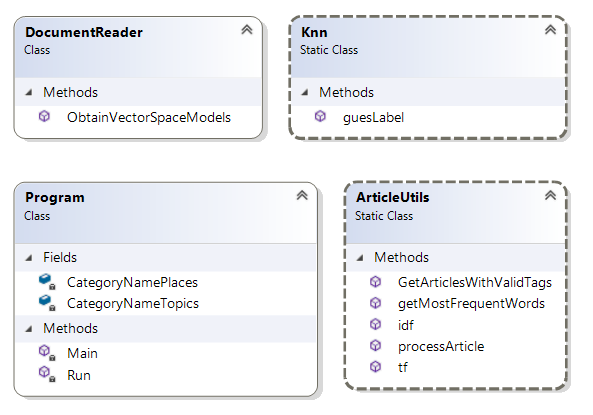
\includegraphics[width=1\textwidth]{/uml1.png}
	\caption{Diagram UML wygenerowany dla klas ogólnych.}
\end{figure}

\item IMetric - interfejs dla metryk, klasy implementujące owy interfejs:
\begin{itemize}
\item ChebyshewMetric -  klasa odpowiedzialna za metrykę Czebyszewa
\item ManhatattanMetric -  klasa odpowiedzialna za metrykę uliczną
\item EuclideanMetric - klasa odpowiedzialna za metrykę euklidesową\\
\end{itemize}

\begin{figure}[H]
	\centering
	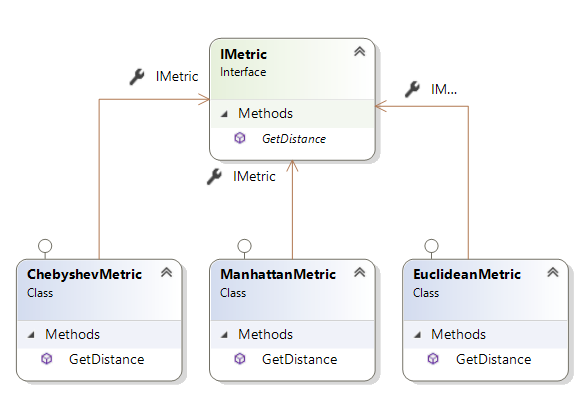
\includegraphics[width=1\textwidth]{/uml2.png}
	\caption{Diagram UML wygenerowany dla klas dotyczących metryk. }
\end{figure}

\item IStemmer - interfejs reprezentujący stemmer
\item Stemmer - reprezentacja stemera
\item EnglishStemer - stemer dla języka angielskiego

\begin{figure}[H]
	\centering
	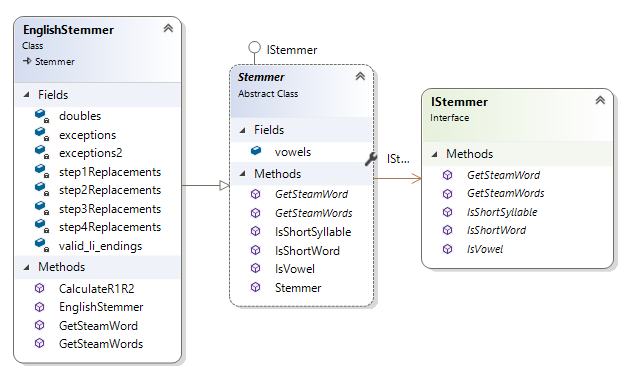
\includegraphics[width=1\textwidth]{/uml3.png}
	\caption{Diagram UML wygenerowany dla klas dotyczących procesu stemizacji.}
\end{figure}

\item Article - klasa reprezentująca pojedyńczy artykuł
\item ProcessedArticle - klasa dziecicząca po Article, reprezentuje przetworzony artykuł


\begin{figure}[H]
	\centering
	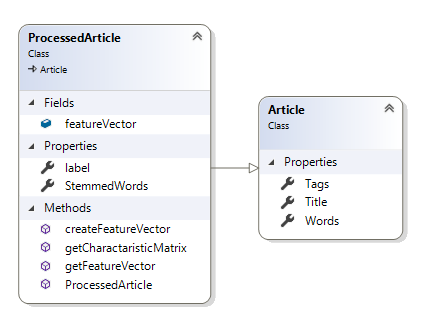
\includegraphics[width=1\textwidth]{/uml4.png}
	\caption{Diagram UML wygenerowany dla klas reprezentujących artykuły.}
\end{figure}

\item IReader - interfejs dla klas wczytujących dane, klasy implementujące owy interfejs:
\begin{itemize}
\item DocumentReader -  klasa odpowiedzialna za wczytanie plików z zestwu \cite{data}
\item CustomReader -  klasa odpowiedzialna za wczytanie plików z przygotowanego przez nas zestawu \cite{our}
\end{itemize}
\end{itemize}

\begin{figure}[H]
	\centering
	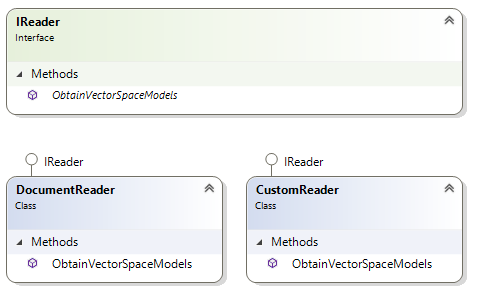
\includegraphics[width=1\textwidth]{/uml5.png}
	\caption{Diagram UML wygenerowany dla klas wczytaujących dane.}
\end{figure}

\section{Materiały i metody}
Klasyfikacja tekstów została wykonana wszystkimi dostępnymi metodami ekstrakcji cech dla wszystkich trzech metryk. Dla każdego przypadku testowego dokonano klasyfikacji tekstu dla k $\in$ \{2, 3, 5, 7, 10, 15, 20\} najbliższych sąsiadów. Wyniki porównano z faktyczną etykietą danego artykułu. \newline

Przyjelismy trzy różne proporcje zbioru treningowego do zbioru testowego, było to:
\begin{itemize}
\item zbiór treningowy 20\%, zbiór testowy 80\%
\item zbiór treningowy 60\%, zbiór testowy 40\%
\item zbiór treningowy 80\%, zbiór testowy 20\%
\end{itemize}

Klasyfikacja dotycząca lokalizacji przeprowadzana była jedynie na danych, których pole places przyjmowało jedną z wartości: west-germany, usa, france, uk, canada, japan.
\newline

Klasyfikacja dotycząca tematów przeprowadzana była jedynie na danych, które pole topics przyjmowało jedną z wartości: gold, cocoa, sugar, coffe, grain.\newline

Danymi jakimi przygotowalimy do analizy były opisy dzieł kultury. Posiadały one jedną kategorię - medium. Pole przyjmowało wartosć: book lub movie.
\section{Wyniki}
\subsection{Term frequency}
%%%%%%
%Euklidesowa
%%%%%%
\subsubsection{Metryka Euklidesowa}
\begin{table}[H]
	\centering
	\begin{tabular}{c c c c} 
		\hline
		\textbf{k} & \textbf{places [\%]} & \textbf{topics [\%]} &  \textbf{medium [\%]} \\ [0.5ex] 
		\hline
		\hline 
2 & 80,3 & 42,4 & 33,8 \\ 
3 & 83,8 & 46,7 & 62,5 \\ 
5 & 84 & 38 & 75 \\ 
7 & 83,6 & 37 & 48,8 \\ 
10 & 83,3 & 35,9 & 37,5 \\ 
15 & 82,8 & 35,9 & 47,5 \\ 
20 & 82 & 35,9 & 48,8 \\ 
		\hline
	\end{tabular}
	\caption{Skuteczność klasyfikacji dla podziału: zbiór treningowy 20\%, zbiór testowy 80\%}
\end{table}

\begin{table}[H]
	\centering
	\begin{tabular}{c c c c} 
		\hline
		\textbf{k} & \textbf{places [\%]} & \textbf{topics [\%]} &  \textbf{medium [\%]} \\ [0.5ex] 
		\hline
		\hline 
2 & 81,3 & 54,3 & 45 \\ 
3 & 85,3 & 58,7 & 47,5 \\ 
5 & 85,4 & 47,8 & 57,5 \\ 
7 & 85,2 & 47,8 & 57,5 \\ 
10 & 84,5 & 45,7 & 52,5 \\ 
15 & 83,6 & 39,1 & 67,5 \\ 
20 & 83,3 & 21,7 & 67,5 \\ 
		\hline
	\end{tabular}
	\caption{Skuteczność klasyfikacji dla podziału: zbiór treningowy 60\%, zbiór testowy 40\%}
\end{table}

\begin{table}[H]
	\centering
	\begin{tabular}{c c c c} 
		\hline
		\textbf{k} & \textbf{places [\%]} & \textbf{topics [\%]} &  \textbf{medium [\%]} \\ [0.5ex] 
		\hline
		\hline 
2 & 84,6 & 47,8 & 75 \\ 
3 & 86,4 & 56,5 & 80 \\ 
5 & 86,9 & 34,8 & 65 \\ 
7 & 87 & 34,8 & 80 \\ 
10 & 86,6 & 43,5 & 70 \\ 
15 & 85,5 & 43,5 & 90 \\ 
20 & 85,6 & 34,8 & 85 \\ 
		\hline
	\end{tabular}
	\caption{Skuteczność klasyfikacji dla podziału: zbiór treningowy 80\%, zbiór testowy 20\%}
\end{table}

%%%%%%
%ulicznej
%%%%%%
\subsubsection{Metryka uliczna}
\begin{table}[H]
	\centering
	\begin{tabular}{c c c c} 
		\hline
		\textbf{k} & \textbf{places [\%]} & \textbf{topics [\%]} &  \textbf{medium [\%]} \\ [0.5ex] 
		\hline
		\hline 
2 & 79,6 & 35,9 & 78,8 \\ 
3 & 82,1 & 48,9 & 62,5 \\ 
5 & 81,8 & 35,9 & 53,8 \\ 
7 & 81,7 & 37 & 53,8 \\ 
10 & 81,8 & 35,9 & 47,5 \\ 
15 & 81,3 & 35,9 & 46,2 \\ 
20 & 80,7 & 35,9 & 48,8 \\ 
		\hline
	\end{tabular}
	\caption{Skuteczność klasyfikacji dla podziału: zbiór treningowy 20\%, zbiór testowy 80\%}
\end{table}

\begin{table}[H]
	\centering
	\begin{tabular}{c c c c} 
		\hline
		\textbf{k} & \textbf{places [\%]} & \textbf{topics [\%]} &  \textbf{medium [\%]} \\ [0.5ex] 
		\hline
		\hline 
2 & 79,9 & 52,2 & 50 \\ 
3 & 83,9 & 54,3 & 47,5 \\ 
5 & 83,7 & 52,2 & 67,5 \\ 
7 & 83,5 & 47,8 & 70 \\ 
10 & 82,7 & 47,8 & 60 \\ 
15 & 82 & 45,7 & 67,5 \\ 
20 & 81,7 & 23,9 & 47,5 \\ 
		\hline
	\end{tabular}
	\caption{Skuteczność klasyfikacji dla podziału: zbiór treningowy 60\%, zbiór testowy 40\%}
\end{table}

\begin{table}[H]
	\centering
	\begin{tabular}{c c c c} 
		\hline
		\textbf{k} & \textbf{places [\%]} & \textbf{topics [\%]} &  \textbf{medium [\%]} \\ [0.5ex] 
		\hline
		\hline 
2 & 84,1 & 47,8 & 65 \\ 
3 & 85,1 & 47,8 & 90 \\ 
5 & 85,6 & 43,5 & 65 \\ 
7 & 84,7 & 30,4 & 80 \\ 
10 & 84,4 & 34,8 & 50 \\ 
15 & 83,6 & 47,8 & 50 \\ 
20 & 83,3 & 39,1 & 85 \\ 
		\hline
	\end{tabular}
	\caption{Skuteczność klasyfikacji dla podziału: zbiór treningowy 80\%, zbiór testowy 20\%}
\end{table}

%%%%%%
%Czebyszewa
%%%%%%
\subsubsection{Metryka Czebyszewa}
\begin{table}[H]
	\centering
	\begin{tabular}{c c c c} 
		\hline
		\textbf{k} & \textbf{places [\%]} & \textbf{topics [\%]} &  \textbf{medium [\%]} \\ [0.5ex] 
		\hline
		\hline 
2 & 80,4 & 42,4 & 53,8 \\ 
3 & 82,4 & 45,7 & 53,8 \\ 
5 & 83,1 & 37 & 68,8 \\ 
7 & 83,2 & 45,7 & 56,2 \\ 
10 & 82,9 & 35,9 & 61,3 \\ 
15 & 82,3 & 35,9 & 52,5 \\ 
20 & 81,6 & 35,9 & 38,8 \\ 
		\hline
	\end{tabular}
	\caption{Skuteczność klasyfikacji dla podziału: zbiór treningowy 20\%, zbiór testowy 80\%}
\end{table}

\begin{table}[H]
	\centering
	\begin{tabular}{c c c c} 
		\hline
		\textbf{k} & \textbf{places [\%]} & \textbf{topics [\%]} &  \textbf{medium [\%]} \\ [0.5ex] 
		\hline
		\hline 
2 & 78,2 & 43,5 & 40 \\ 
3 & 82,3 & 47,8 & 57,5 \\ 
5 & 82,8 & 45,7 & 77,5 \\ 
7 & 83 & 45,7 & 80 \\ 
10 & 82,8 & 43,5 & 45 \\ 
15 & 82,6 & 32,6 & 60 \\ 
20 & 82 & 28,3 & 50 \\ 
		\hline
	\end{tabular}
	\caption{Skuteczność klasyfikacji dla podziału: zbiór treningowy 60\%, zbiór testowy 40\%}
\end{table}

\begin{table}[H]
	\centering
	\begin{tabular}{c c c c} 
		\hline
		\textbf{k} & \textbf{places [\%]} & \textbf{topics [\%]} &  \textbf{medium [\%]} \\ [0.5ex] 
		\hline
		\hline 
2 & 82,1 & 30,4 & 60 \\ 
3 & 84,6 & 39,1 & 70 \\ 
5 & 84,7 & 26,1 & 75 \\ 
7 & 84,5 & 30,4 & 45 \\ 
10 & 84,4 & 30,4 & 40 \\ 
15 & 84,3 & 26,1 & 75 \\ 
20 & 83,3 & 26,1 & 60 \\ 
		\hline
	\end{tabular}
	\caption{Skuteczność klasyfikacji dla podziału: zbiór treningowy 80\%, zbiór testowy 20\%}
\end{table}


\subsection{Term frequency - podsumowanie wykresami}
%%%PLACES
\begin{figure}[H]
	\centering
	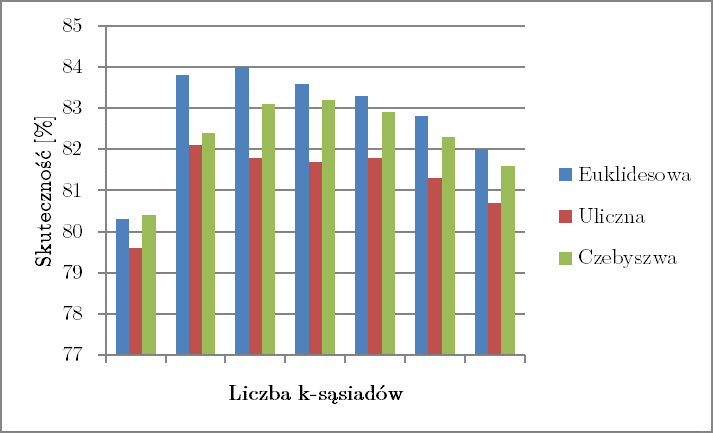
\includegraphics[width=1\textwidth]{/results/TF_20_places.png}
	\caption{Dane z tabel 1-9 dla kategorii places, zbiór treningowy 20\%, zbiór testowy 80\%}
\end{figure}
\begin{figure}[H]
	\centering
	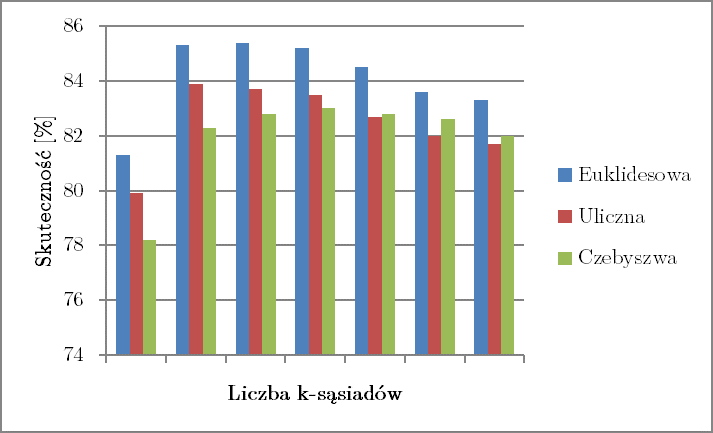
\includegraphics[width=1\textwidth]{/results/TF_60_places.png}
	\caption{Dane z tabel 1-9 dla kategorii places, zbiór treningowy 60\%, zbiór testowy 40\%}
\end{figure}
\begin{figure}[H]
	\centering
	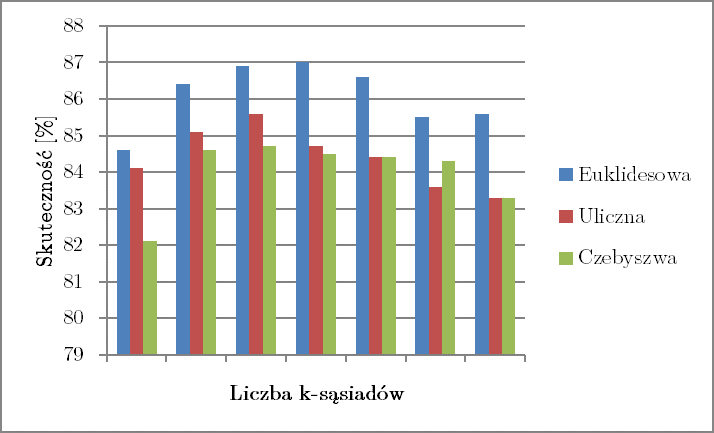
\includegraphics[width=1\textwidth]{/results/TF_80_places.png}
	\caption{Dane z tabel 1-9 dla kategorii places, zbiór treningowy 80\%, zbiór testowy 20\%}
\end{figure}
%%%Topics
\begin{figure}[H]
	\centering
	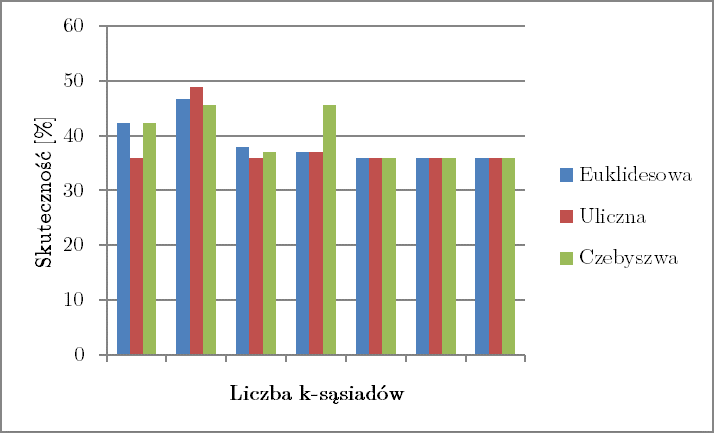
\includegraphics[width=1\textwidth]{/results/TF_20_topics.png}
	\caption{Dane z tabel 1-9 dla kategorii topics, zbiór treningowy 20\%, zbiór testowy 80\%}
\end{figure}
\begin{figure}[H]
	\centering
	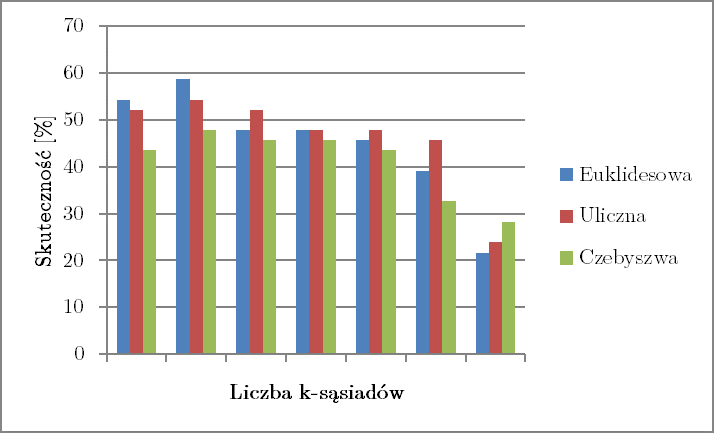
\includegraphics[width=1\textwidth]{/results/TF_60_topics.png}
	\caption{Dane z tabel 1-9 dla kategorii topics, zbiór treningowy 60\%, zbiór testowy 40\%}
\end{figure}
\begin{figure}[H]
	\centering
	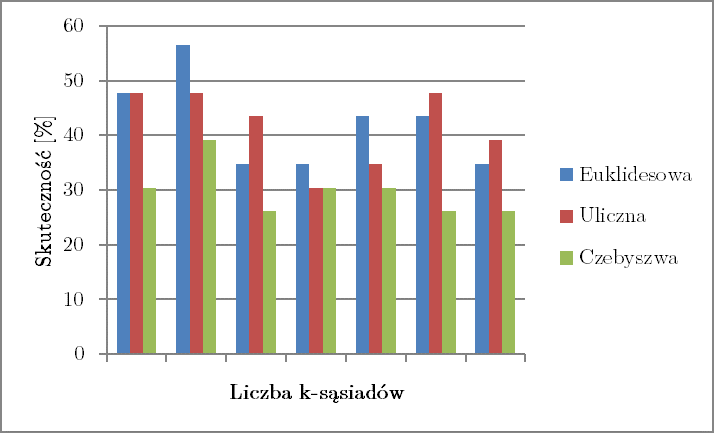
\includegraphics[width=1\textwidth]{/results/TF_80_topics.png}
	\caption{Dane z tabel 1-9 dla kategorii topics, zbiór treningowy 80\%, zbiór testowy 20\%}
\end{figure}
%%%MEDIUM
\begin{figure}[H]
	\centering
	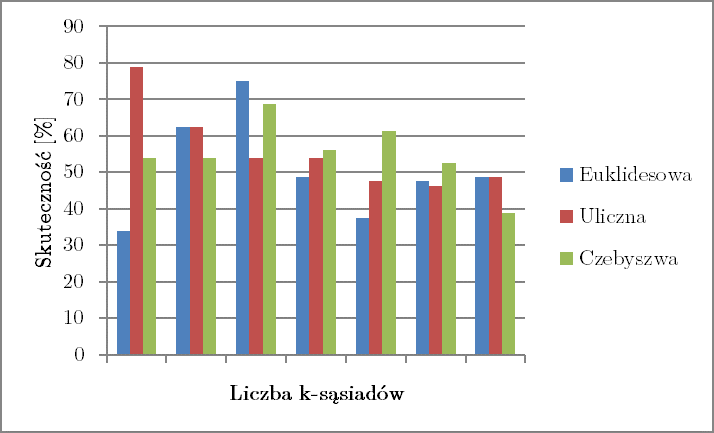
\includegraphics[width=1\textwidth]{/results/TF_20_medium.png}
	\caption{Dane z tabel 1-9 dla kategorii medium, zbiór treningowy 20\%, zbiór testowy 80\%}
\end{figure}
\begin{figure}[H]
	\centering
	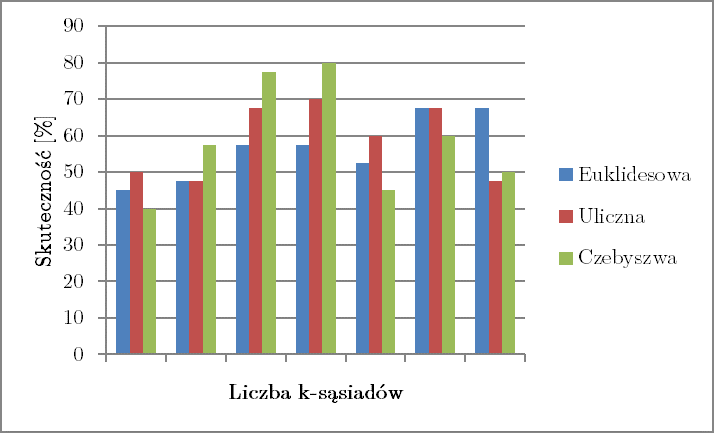
\includegraphics[width=1\textwidth]{/results/TF_60_medium.png}
	\caption{Dane z tabel 1-9 dla kategorii medium, zbiór treningowy 60\%, zbiór testowy 40\%}
\end{figure}
\begin{figure}[H]
	\centering
	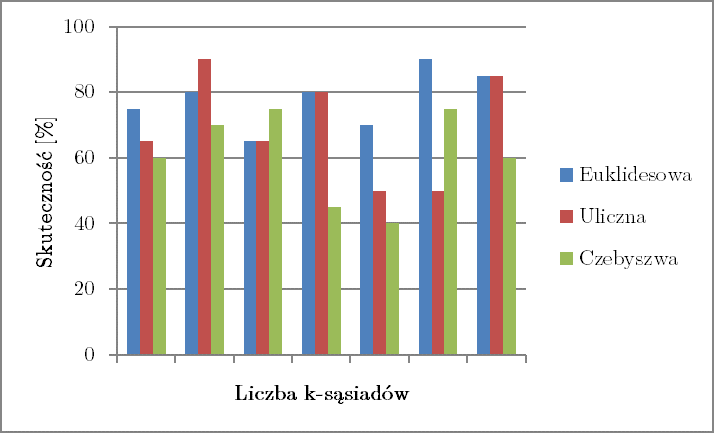
\includegraphics[width=1\textwidth]{/results/TF_80_medium.png}
	\caption{Dane z tabel 1-9 dla kategorii medium, zbiór treningowy 80\%, zbiór testowy 20\%}
\end{figure}

%%%%%%%%%%%%%%%%%%%%%%%%%%%%%%%%%%%%%%%%%%%%%%%%%%%%%%%%%%%%%%%%%%%%%%%%%%%%
%%%%%
%%%%%%%%%%%%%%%%%%%%%%%%%%%%%%%%%%%%%%%%%%%%%%%%%%%%%%%%%%%%%%%%%%%%%%%%%%%%
\subsection{Inverse document frequency}

%%%%%%
%Euklidesowa
%%%%%%
\subsubsection{Metryka Euklidesowa}
\begin{table}[H]
	\centering
	\begin{tabular}{c c c c} 
		\hline
		\textbf{k} & \textbf{places [\%]} & \textbf{topics [\%]} &  \textbf{medium [\%]} \\ [0.5ex] 
		\hline
		\hline 
2 & 78,7 & 32,6 & 57,5 \\ 
3 & 82,6 & 31,5 & 43,8 \\ 
5 & 82,9 & 29,3 & 65 \\ 
7 & 82,3 & 33,7 & 66,2 \\ 
10 & 81,7 & 33,7 & 51,2 \\ 
15 & 81,3 & 35,9 & 46,2 \\ 
20 & 81 & 35,9 & 46,2 \\ 
		\hline
	\end{tabular}
	\caption{Skuteczność klasyfikacji dla podziału: zbiór treningowy 20\%, zbiór testowy 80\%}
\end{table}

\begin{table}[H]
	\centering
	\begin{tabular}{c c c c} 
		\hline
		\textbf{k} & \textbf{places [\%]} & \textbf{topics [\%]} &  \textbf{medium [\%]} \\ [0.5ex] 
		\hline
		\hline 
2 & 78,6 & 34,8 & 57,5 \\ 
3 & 82,3 & 32,6 & 62,5 \\ 
5 & 83,5 & 28,3 & 45 \\ 
7 & 83,7 & 28,3 & 67,5 \\ 
10 & 83,4 & 28,3 & 30 \\ 
15 & 82,8 & 21,7 & 42,5 \\ 
20 & 82,6 & 26,1 & 45 \\ 
		\hline
	\end{tabular}
	\caption{Skuteczność klasyfikacji dla podziału: zbiór treningowy 60\%, zbiór testowy 40\%}
\end{table}

\begin{table}[H]
	\centering
	\begin{tabular}{c c c c} 
		\hline
		\textbf{k} & \textbf{places [\%]} & \textbf{topics [\%]} &  \textbf{medium [\%]} \\ [0.5ex] 
		\hline
		\hline 
2 & 80,5 & 30,4 & 35 \\ 
3 & 83,8 & 34,8 & 65 \\ 
5 & 83,8 & 21,7 & 55 \\ 
7 & 83,8 & 26,1 & 45 \\ 
10 & 83,5 & 26,1 & 50 \\ 
15 & 83,7 & 43,5 & 50 \\ 
20 & 83,1 & 34,8 & 70 \\ 
		\hline
	\end{tabular}
	\caption{Skuteczność klasyfikacji dla podziału: zbiór treningowy 80\%, zbiór testowy 20\%}
\end{table}

%%%%%%
%ulicznej
%%%%%%
\subsubsection{Metryka uliczna}
\begin{table}[H]
	\centering
	\begin{tabular}{c c c c} 
		\hline
		\textbf{k} & \textbf{places [\%]} & \textbf{topics [\%]} &  \textbf{medium [\%]} \\ [0.5ex] 
		\hline
		\hline 
2 & 77,8 & 31,5 & 50 \\ 
3 & 81,2 & 34,8 & 63,7 \\ 
5 & 81,7 & 33,7 & 52,5 \\ 
7 & 81,3 & 34,8 & 45 \\ 
10 & 81,2 & 35,9 & 57,5 \\ 
15 & 81 & 35,9 & 47,5 \\ 
20 & 81 & 35,9 & 47,5 \\ 
		\hline
	\end{tabular}
	\caption{Skuteczność klasyfikacji dla podziału: zbiór treningowy 20\%, zbiór testowy 80\%}
\end{table}

\begin{table}[H]
	\centering
	\begin{tabular}{c c c c} 
		\hline
		\textbf{k} & \textbf{places [\%]} & \textbf{topics [\%]} &  \textbf{medium [\%]} \\ [0.5ex] 
		\hline
		\hline 
2 & 78,8 & 19,6 & 60 \\ 
3 & 81,8 & 19,6 & 52,5 \\ 
5 & 82,6 & 19,6 & 65 \\ 
7 & 82,8 & 17,4 & 67,5 \\ 
10 & 82,2 & 19,6 & 50 \\ 
15 & 81,9 & 19,6 & 70 \\ 
20 & 81,5 & 26,1 & 75 \\ 
		\hline
	\end{tabular}
	\caption{Skuteczność klasyfikacji dla podziału: zbiór treningowy 60\%, zbiór testowy 40\%}
\end{table}

\begin{table}[H]
	\centering
	\begin{tabular}{c c c c} 
		\hline
		\textbf{k} & \textbf{places [\%]} & \textbf{topics [\%]} &  \textbf{medium [\%]} \\ [0.5ex] 
		\hline
		\hline 
2 & 79,2 & 26,1 & 50 \\ 
3 & 83,3 & 30,4 & 50 \\ 
5 & 83,4 & 26,1 & 45 \\ 
7 & 83,3 & 21,7 & 60 \\ 
10 & 82,9 & 26,1 & 65 \\ 
15 & 82,8 & 39,1 & 45 \\ 
20 & 82,2 & 26,1 & 70 \\ 

		\hline
	\end{tabular}
	\caption{Skuteczność klasyfikacji dla podziału: zbiór treningowy 80\%, zbiór testowy 20\%}
\end{table}

%%%%%%
%Czebyszewa
%%%%%%
\subsubsection{Metryka Czebyszewa}
\begin{table}[H]
	\centering
	\begin{tabular}{c c c c} 
		\hline
		\textbf{k} & \textbf{places [\%]} & \textbf{topics [\%]} &  \textbf{medium [\%]} \\ [0.5ex] 
		\hline
		\hline 
2 & 77,6 & 31,5 & 62,5 \\ 
3 & 80,7 & 31,5 & 51,2 \\ 
5 & 81,5 & 40,2 & 58,8 \\ 
7 & 81,2 & 33,7 & 70 \\ 
10 & 81 & 34,8 & 47,5 \\ 
15 & 80,5 & 35,9 & 57,5 \\ 
20 & 79,6 & 35,9 & 50 \\ 
		\hline
	\end{tabular}
	\caption{Skuteczność klasyfikacji dla podziału: zbiór treningowy 20\%, zbiór testowy 80\%}
\end{table}

\begin{table}[H]
	\centering
	\begin{tabular}{c c c c} 
		\hline
		\textbf{k} & \textbf{places [\%]} & \textbf{topics [\%]} &  \textbf{medium [\%]} \\ [0.5ex] 
		\hline
		\hline 
2 & 79,8 & 41,3 & 47,5 \\ 
3 & 81,8 & 63 & 42,5 \\ 
5 & 81,6 & 28,3 & 62,5 \\ 
7 & 81,7 & 39,1 & 70 \\ 
10 & 81,6 & 34,8 & 65 \\ 
15 & 81,6 & 23,9 & 45 \\ 
20 & 81,5 & 23,9 & 52,5 \\ 
		\hline
	\end{tabular}
	\caption{Skuteczność klasyfikacji dla podziału: zbiór treningowy 60\%, zbiór testowy 40\%}
\end{table}

\begin{table}[H]
	\centering
	\begin{tabular}{c c c c} 
		\hline
		\textbf{k} & \textbf{places [\%]} & \textbf{topics [\%]} &  \textbf{medium [\%]} \\ [0.5ex] 
		\hline
		\hline 
2 & 79,1 & 43,5 & 80 \\ 
3 & 82,4 & 39,1 & 60 \\ 
5 & 81,6 & 26,1 & 40 \\ 
7 & 81,7 & 30,4 & 50 \\ 
10 & 81,9 & 26,1 & 55 \\ 
15 & 82,2 & 26,1 & 60 \\ 
20 & 82,1 & 26,1 & 65 \\ 
		\hline
	\end{tabular}
	\caption{Skuteczność klasyfikacji dla podziału: zbiór treningowy 80\%, zbiór testowy 20\%}
\end{table}

\subsection{Inverse document frequency - podsumowanie wykresami}
%%%PLACES
\begin{figure}[H]
	\centering
	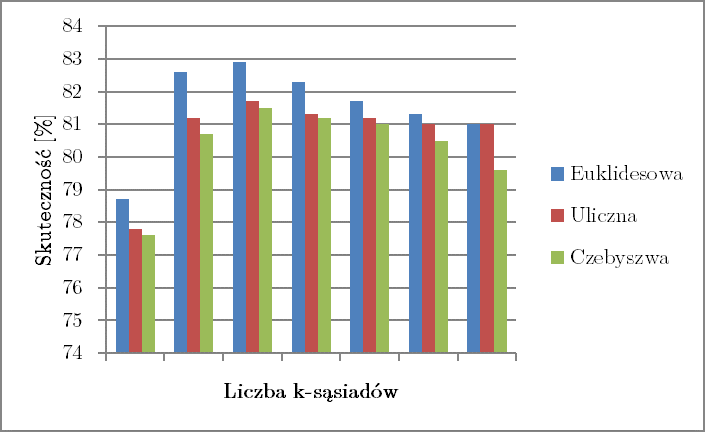
\includegraphics[width=1\textwidth]{/results/IDF_20_places.png}
	\caption{Dane z tabel 1-9 dla kategorii places, zbiór treningowy 20\%, zbiór testowy 80\%}
\end{figure}
\begin{figure}[H]
	\centering
	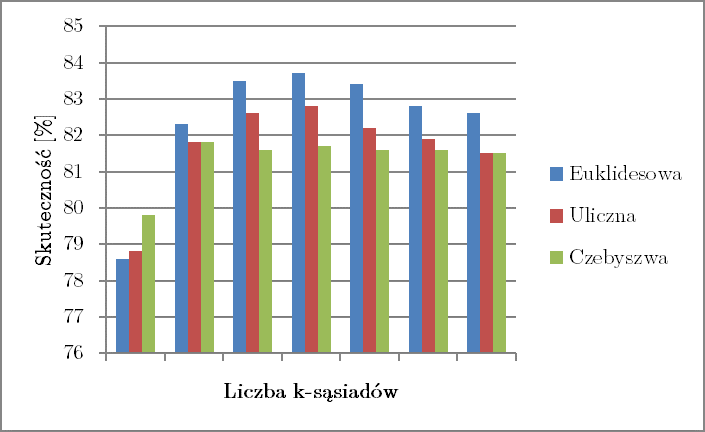
\includegraphics[width=1\textwidth]{/results/IDF_60_places.png}
	\caption{Dane z tabel 1-9 dla kategorii places, zbiór treningowy 60\%, zbiór testowy 40\%}
\end{figure}
\begin{figure}[H]
	\centering
	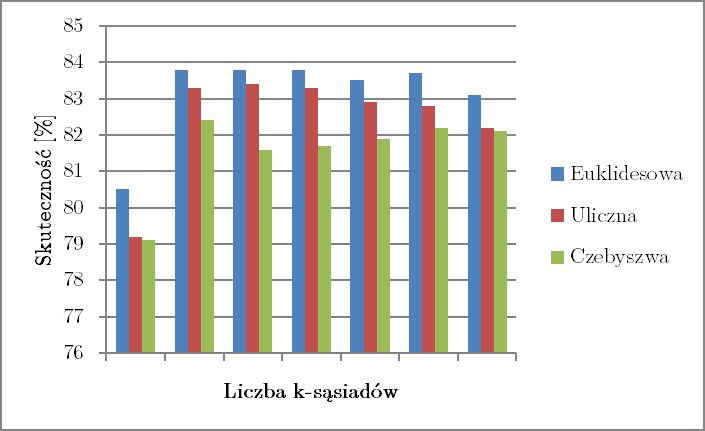
\includegraphics[width=1\textwidth]{/results/IDF_80_places.png}
	\caption{Dane z tabel 1-9 dla kategorii places, zbiór treningowy 80\%, zbiór testowy 20\%}
\end{figure}
%%%Topics
\begin{figure}[H]
	\centering
	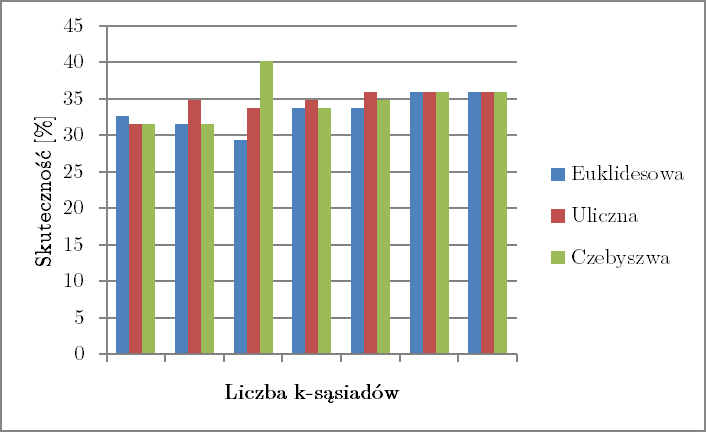
\includegraphics[width=1\textwidth]{/results/IDF_20_topics.png}
	\caption{Dane z tabel 1-9 dla kategorii topics, zbiór treningowy 20\%, zbiór testowy 80\%}
\end{figure}
\begin{figure}[H]
	\centering
	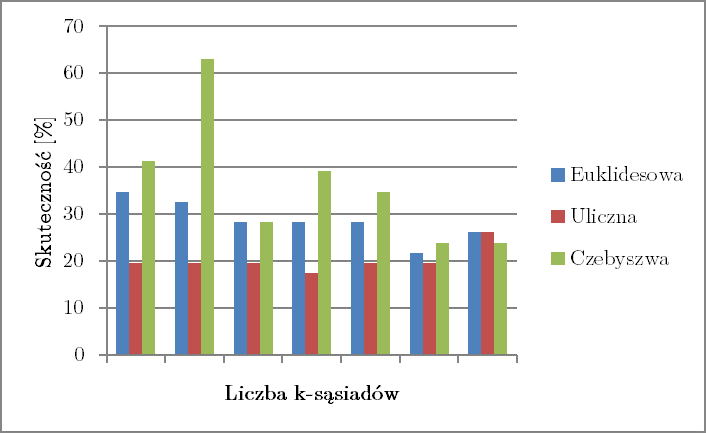
\includegraphics[width=1\textwidth]{/results/IDF_60_topics.png}
	\caption{Dane z tabel 1-9 dla kategorii topics, zbiór treningowy 60\%, zbiór testowy 40\%}
\end{figure}
\begin{figure}[H]
	\centering
	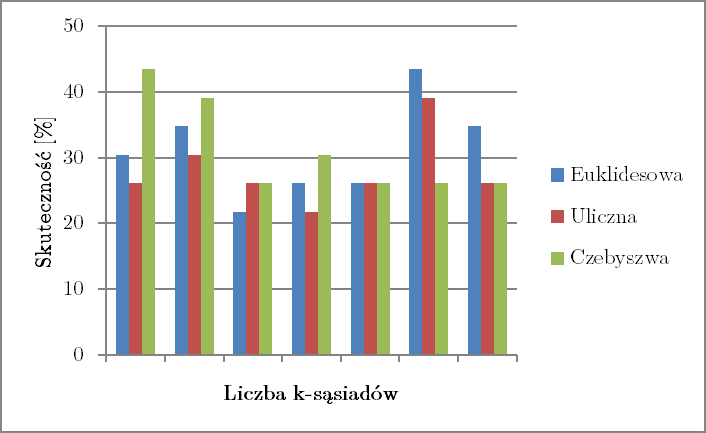
\includegraphics[width=1\textwidth]{/results/IDF_80_topics.png}
	\caption{Dane z tabel 1-9 dla kategorii topics, zbiór treningowy 80\%, zbiór testowy 20\%}
\end{figure}
%%%MEDIUM
\begin{figure}[H]
	\centering
	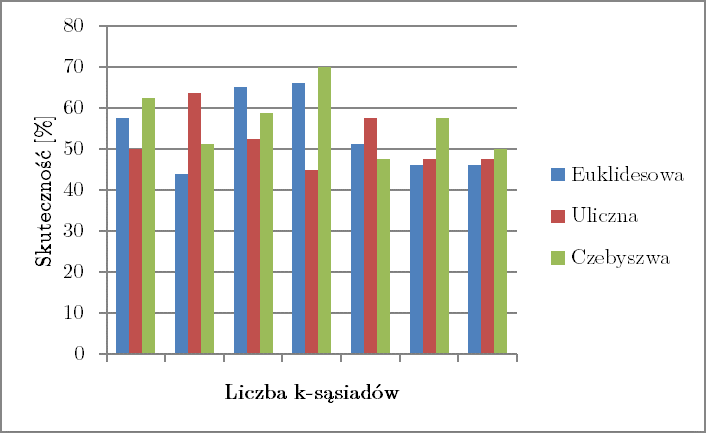
\includegraphics[width=1\textwidth]{/results/IDF_20_medium.png}
	\caption{Dane z tabel 1-9 dla kategorii medium, zbiór treningowy 20\%, zbiór testowy 80\%}
\end{figure}
\begin{figure}[H]
	\centering
	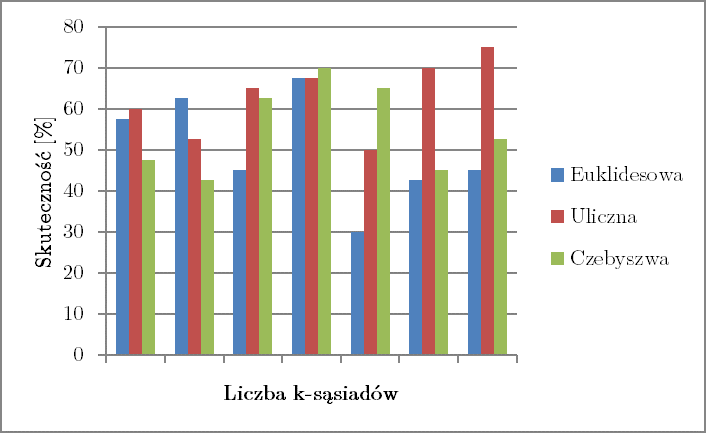
\includegraphics[width=1\textwidth]{/results/IDF_60_medium.png}
	\caption{Dane z tabel 1-9 dla kategorii medium, zbiór treningowy 60\%, zbiór testowy 40\%}
\end{figure}
\begin{figure}[H]
	\centering
	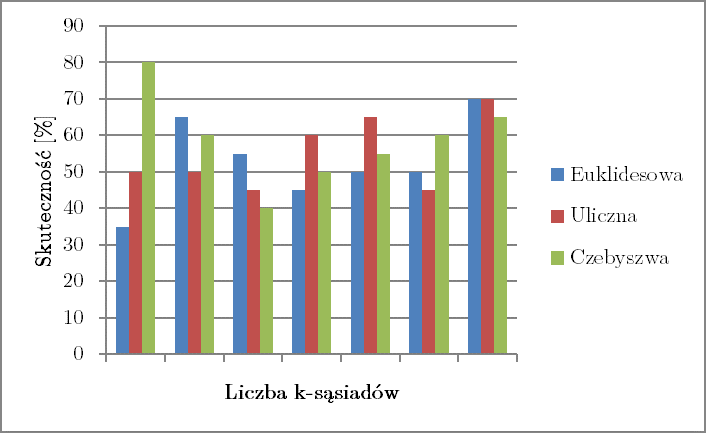
\includegraphics[width=1\textwidth]{/results/IDF_80_medium.png}
	\caption{Dane z tabel 1-9 dla kategorii medium, zbiór treningowy 80\%, zbiór testowy 20\%}
\end{figure}

\section{Dyskusja}



{\color{blue}
Sekcja ta powinna zawierać dokładną interpretację uzyskanych wyników
eksperymentów wraz ze szczegółowymi wnioskami z nich płynącymi. Najcenniejsze
są, rzecz jasna, wnioski o charakterze uniwersalnym, które mogą być istotne
przy innych, podobnych zadaniach. Należy również omówić i wyjaśnić wszystkie
napotakane problemy (jeśli takie były). Każdy wniosek powinien mieć poparcie
we wcześniej przeprowadzonych eksperymentach (odwołania do konkretnych
wyników). Jest to jedna z najważniejszych sekcji tego sprawozdania, gdyż
prezentuje poziom zrozumienia badanego problemu.}
\section{Wnioski}
\begin{itemize}
\item Wniosek1
\item Wniosek2
\item Wniosek3
\end{itemize}

\begin{thebibliography}{}
\bibitem{adam}
Methods for the linguistic summarization of data - aplications of fuzzy sets and their extensions, Adam Niewiadomski, Akademicka Oficyna Wydawnicza EXIT, Warszawa 2008
\bibitem{stop}
https://github.com/hklemp/dotnet-stop-words
\bibitem{stemmer}
http://snowball.tartarus.org/algorithms/english/stemmer.html
\bibitem{data}
https://archive.ics.uci.edu/ml/datasets/Reuters-21578+Text+Categorization+Collection
\bibitem{our}
https://github.com/jurczewski/KSR/blob/master/Zad1/Zad1/Data/ours.sgm
\end{thebibliography}
\end{document}
